\section{RT simulation and CHiL testing}\label{sec:rtchil}

All analyses in this section have been conducted with \textit{Release} builds if not mentioned otherwise explicitly (cf. Section \ref{sec:STM32CubeIDE}).

\subsection{CHiL experimental setup}

\paragraph{Schematics and wiring:} To perform CHiL tests, Figure \ref{fig:wiring-diagram} shows how the microcontrollers have been wired together along with an Analog Discovery 3\footnote{\tiny{\url{https://digilent.com/shop/analog-discovery-3/}}}, a multi-functional test and measurement device (labeled (M)). On the left hand side, the NUCLEO-L476RG, labeled (C), serves as the \controller{} running the PSS eFMU (from the model in Figure \ref{fig:pssvariants}~(D)), while on the right hand side the NUCLEO-H723ZG, labeled (P), acts as the \plant{} running the other eFMU (from the model in Figure \ref{fig:g4chil}).

\begin{figure}[h]
    \centerline{\includesvg[width=0.975\columnwidth]{./figures/setup-path.svg}}
    \vspace{-2ex}
    \caption{CHiL experimental setup wired to record measurement data from experiments using the Analog Discovery 3.}
    \label{fig:wiring-diagram}
    \vspace{-1ex}
\end{figure}

The speed output signal \texttt{w} of the \plant{}, in Figure \ref{fig:g4chil}, is now physically obtained from Figure \ref{fig:wiring-diagram}(P) (the NUCLEO-H723ZG) on pin \texttt{D13}. It is connected with a yellow wire to both the measurement channel \texttt{C1} of the Analog Discovery Board 3 (M) and to pin \texttt{A5} of the \controller{}, the NUCLEO-L476RG, labeled (C) in Figure \ref{fig:wiring-diagram}. Similarly, the output signal \texttt{vf} of the \controller{} in Figure \ref{fig:pssvariants}~(D)) is obtained from the NUCLEO-L476RG in Figure \ref{fig:wiring-diagram}(C) from pin \texttt{A2}. It is then connected with green wires to both the measurement channel \texttt{C2} of the Analog Discovery Board 3 and to pin \texttt{A0} of the \plant{}, the NUCLEO-H723ZG.

\paragraph{Interactive fault injection, stabilizer toggling, and resetting:} In traditional offline Modelica simulations, events like faults, reinitialization, or enabling or disabling a controller are typically triggered by absolute time components (e.g., the \texttt{faultTimer} in our offline simulation models of the CHiL setup, shown in Figure \ref{fig:chilmodels}). In a continuous HiL environment, absolute time based events are problematic however; there might be no well-defined, synchronized global clock for all devices, multiple consecutive test runs require synchronous resetting of all boards, and interactive testing is hampered. For these reasons, we decided for interactive, onboard button based, event triggering.

Manual \plant{} faults can be triggered by pushing the blue ``User Button'' on the NUCLEO-H723ZG, which is labeled \texttt{B1} on the bottom right of Figure \ref{fig:wiring-diagram}. Pressing the button pulls the GPIO pin high, instantly activating the fault dynamics of the \plant{} eFMU, while releasing it clears the fault, allowing for interactive, repeatable time-domain testing.

In case of the \controller{}, the corresponding ``User Button'' is configured to engage or disengage the eFMU itself. When the \controller{} button \texttt{B1}, on the left of Figure \ref{fig:wiring-diagram}, is pressed, it will ``turn-on'' the PSS, giving an output driven by the eFMU, and pressing it again will ``turn-off'' the PSS, giving a constant output.

Both boards, the L476RG and the H723ZG, can be individually reset using the buttons labeled \texttt{B2}, on the left hand side for the \controller{} and on the bottom right hand side for the \plant{}.

\paragraph{Analog Discovery 3 oscilloscope and network analysis:} The Analog Discovery 3 interfaces with Digilent's WaveForms\footref{fnt:waveforms} software package. This software is capable of acquiring oscilloscope measurements through two analog channels (see \texttt{C1} and \texttt{C2} in Figure \ref{fig:wiring-diagram}), allowing real-time analysis of the analog signals used by microcontrollers during experiments. Additionally, the Analog Discovery 3 includes a waveform generator, allowing for test signal injection into the Nucleo-64/144 boards so that their functionality could be tested independently. The WaveForms software also includes a network analysis tool, employing both the oscilloscope and waveform generator hardware features. This tool allows for the frequency dependent amplitude and phase responses of the circuit under test to be captured easily. This is achieved by connecting the waveform generator, \texttt{W1} in Figure \ref{fig:wiring-diagram}, and one analog probe, \texttt{C1}, to the input of the system, with the second analog probe, \texttt{C2} connected to the output of the system. Through this network analysis function, frequency response plots were generated and compared with the Bode plots generated by linearizing the Modelica models.

\paragraph{Full closed-loop network analysis setup:} Because the experimental CHiL setup includes two embedded boards in closed-loop, it is desirable to verify the frequency response characteristics of this closed-loop system as well. Figure \ref{fig:closed-loop-simulation} shows the Dymola model that was used to compare with the hardware-based closed-loop test.

\begin{figure}[t!]
    \centerline{\includesvg[width=0.95\columnwidth]{./figures/IOCL.svg}}
    \caption{Closed-loop model with input and output interfaces to compare with frequency response tests.}
    \label{fig:closed-loop-simulation}
    \vspace{-1ex}
\end{figure}

\begin{figure*}[t!]
    \centerline{\includesvg[width=1.5\columnwidth]{./figures/closed_loop_wiring_diagram_larger.svg}}
    \vspace{-2ex}
    \caption{Closed-Loop wiring diagram for network analysis experiments with Analog Discovery 3.}
    \label{fig:closed-loop-wiring-diagram}
    \vspace{-2ex}
\end{figure*}

To obtain measurements of the closed-loop frequency response without violating the electrical constraints of the STM32 hardware, a custom signal injection circuit was required. The STM32's Analog-to-Digital Converter (ADC) operates on a single-supply 3.3 V logic level and cannot physically process negative voltages. Injecting a standard 0 V offset AC sweep directly into the ADC would result in severe signal clipping and non-linear distortion. As shown in the schematic in Figure \ref{fig:closed-loop-wiring-diagram}, a non-inverting summing amplifier was constructed using a MAX474 operational amplifier. The adder takes the nominal steady-state speed output of the \plant{}, which rests at a flat 1.0 V DC, and sums it with the small AC signal ($\pm50$ mV, 0 V offset) generated by the Analog Discovery 3 from pin \texttt{W1}. This outputs a safely biased signal fluctuating between 0.95 V and 1.05 V into the \controller{}'s ADC. By measuring the injected stimulus on channel \texttt{C1} and the \plant{}'s speed output on channel \texttt{C2}, the true closed-loop transfer function was empirically captured.

\subsection{Results and analyses}\label{sec:results-and-analyses}

\paragraph{Time-domain analyses:} To establish a baseline, the system was first tested having the PSS eFMU functions disengaged. Figure \ref{fig:time-plot-no-pss} displays the time domain plot of the generator's speed deviation (blue trace) when subjected to a fault without engaged \controller{}. In this case, the \plant{} essentially behaving as an undamped pendulum, exhibiting sustained electromechanical oscillations, which are further excited following a later fault triggering making the \plant{} unstable.

\begin{figure}[t!]
   \centerline{\includesvg[width=0.975\columnwidth]{./figures/f19-exp-pss-disengaged.svg}}
    \caption{Experiment with the PSS disengaged. Orange: PSS output voltage (pu) from the Nucle-L476RG, Blue: scaled speed from the NUCLEO-H723ZG. Red dashed: fault applied.}
    \label{fig:time-plot-no-pss}
    \vspace{-1ex}
\end{figure}

The system's response with the tuned \controller{} active in the control loop is shown in Figure \ref{fig:time-plot-with-pss}. The injection of the \controller{} voltage (shown in orange) provides immediate active damping. The generator speed (shown in blue) damps to a steady state within seconds. Furthermore, the active \controller{} allowed the physical hardware simulation to recover successfully from a $\pm0.2$ pu speed deviation, whereas the uncompensated \plant{} became unstable when subjected to deviations greater than $\pm0.1$ pu.

\begin{figure}[t!]
    \centerline{\includesvg[width=0.975\columnwidth]{./figures/f20-exp-pss-engaged.svg}}
    \caption{Experiment with PSS engaged. Orange: PSS output voltage (pu) from the NUCLEO-L476RG, Blue: scaled speed from the NUCLEO-H723ZG. Red dashed: fault applied. Magenta dotted: reset of both boards.}
    \label{fig:time-plot-with-pss}
    \vspace{-2ex}
\end{figure}

For both experiments in Figures \ref{fig:time-plot-no-pss} \& \ref{fig:time-plot-with-pss}, excessively large faults were applied to the system (the \plant{} \texttt{B1} button was held down for long periods); evident where the generator speed would become unstable, rapidly increasing, and eventually saturating. This is because the \controller{} has a limited operational window of generator speeds it can stabilize.

\paragraph{Frequency-domain analyses:} The WaveForms network analyzer was configured to perform logarithmic frequency sweeps from 0.15 to 100 Hz. A signal amplitude of 50 mV was selected for the waveform generator to ensure that the \plant{} AVR limits were never reached during the test.

\begin{figure}[t!]
    \centerline{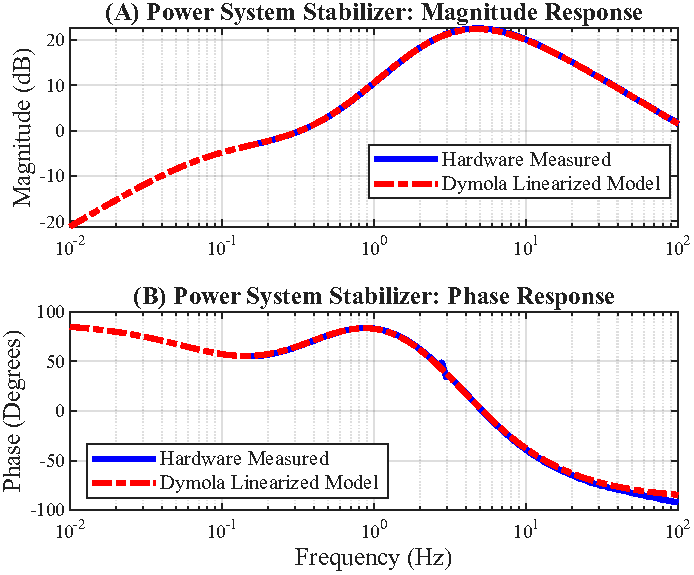
\includegraphics[width=0.9\columnwidth]{./figures/sec06-PSS-bode.pdf}}
    \vspace{-2ex}
    \caption{Frequency response of the \controller{}. Blue: NUCLEO-L476RG running the eFMU, Red: Dymola linearized model.}
    \label{fig:freq-plot-pss}
    \vspace{-2ex}
\end{figure}

First, an open-loop frequency response experiment was conducted on the \controller{}. Figure \ref{fig:freq-plot-pss} shows the Bode plot obtained by analyzing the linear model generated from Dymola (by linearizing the model in Figure \ref{fig:pssvariants}(D)) in a red dashed line, along with the measured Bode plot measured from the hardware (blue line). The excellent agreement of both traces confirms that the \controller{} simulation is running as expected. If the timer's time step on the NUCLEO-L476RG was not configured to exactly match the time step set in Dymola's eFMU export, the entire graph would maintain the same shape but shift horizontally along the frequency axis. 

\begin{figure}[t!]
    \centerline{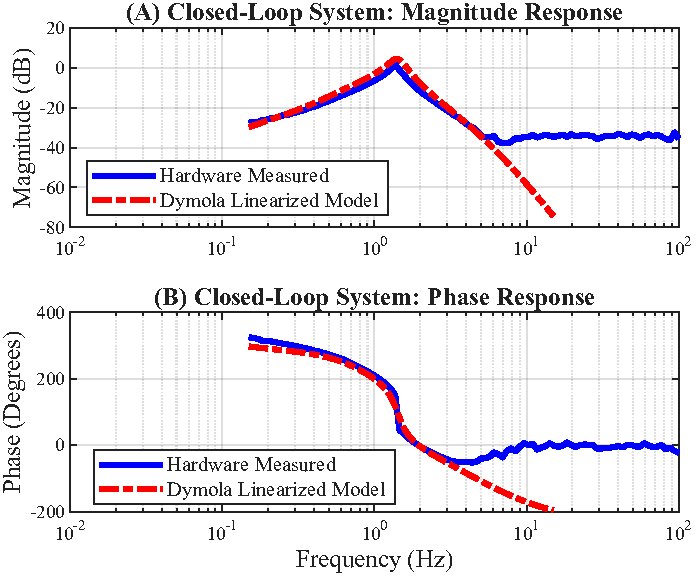
\includegraphics[width=0.9\columnwidth]{./figures/sec06-CLsys-bode.pdf}}
    \vspace{-2ex}
    \caption{Frequency response of the closed-loop test. Blue: hardware measurements, Red: Dymola linearized model.}
    \label{fig:freq-plot-cl}
    \vspace{-2ex}
\end{figure}

The closed-loop experiment was then conducted. Figure \ref{fig:freq-plot-cl} shows the Bode plot obtained by linearizing the model in Figure \ref{fig:closed-loop-simulation} in Dymola, and the one measured during the experiment. Although there is no perfect alignment in this case, they match closely enough to indicate that the eFMU is producing results that are highly consistent with the offline simulation. Measurements at $\approx$5 Hz appear to flatten according to Figure \ref{fig:freq-plot-cl}~(B), albeit with a jagged nature due to noise. This is likely due to the Analog Discovery 3 hitting its measurement noise floor, where it cannot accurately resolve the frequency response at that level of sensitivity anymore, and the limitations of the used onboard ADCs and DACs.

\paragraph{Computation time analyses:} A critical requirement of the CHiL tests is to validate that there are no real-time violations (called overruns), i.e., the \controller{} and \plant{} always finish computing a sampling before a subsequent timer interrupt triggers, requesting the next sampling cycle to be evaluated. To verify this, onboard LED 2 on either board is used (cf. Figure \ref{fig:wiring-diagram}); whenever an overrun is detected, it turns on green for 30 s for the \controller{} or yellow for 5 s for the \plant{}. Note, that LEDs are also used for indicating error signals from the eFMU production codes (like when the embedded linear solver failed due to a singularity). Since the NUCLEO-L476RG of the \controller{} only has LED 2 available for user programs, it is shared for overrun detection and error signals; thus, if it turns on it could be either an overrun or an error signal. For the NUCLEO-H723ZG of the \plant{}, LED 3 (red) is used to indicate error signals.

Although LEDs are helpful for diagnostic purposes, they do not provide any information to which degree real-time requirements are satisfied (if they are); but the headroom for potential additional computations is a good indication if the chosen board is a good fit considering also some security-buffer in case future model changes may cause reasonable additional computational-effort. Therefore, digital GPIO pins were configured to turn on high at the exact start of sampling and to turn off low immediately upon completion (labeled \texttt{D12} in Figure \ref{fig:wiring-diagram} for the \controller{} and \texttt{D2} for the \plant{}). By monitoring the respective pin of either board with the oscilloscope, the true computation time, \texttt{calcTime}, can be physically measured. To be able to plot the computation time relative to the sampling period of that board, timer interrupts are also toggling a separate digital GPIO pin, the \texttt{stepSize} (labeled \texttt{D11} in Figure \ref{fig:wiring-diagram} for the \controller{} and \texttt{D3} for the \plant{}).

\begin{figure}[t!]
    \centerline{\includesvg[width=0.975\columnwidth]{./figures/Fig23.svg}}
    \vspace{-2ex}
    \caption{Computation time (blue) and sampling timer (orange) of the NUCLEO-H723ZG executing the 32-bit floating-point precision eFMI production code (\textit{Release} build) of the \plant{} under (A) steady state, (B) sustained fault injection.}
    \label{fig:calc-time}
    \vspace{-2ex}
\end{figure}

%----------------------------------------------
% Computation time measurements
%----------------------------------------------
% Plant, 32-bit FP, no sustained fault
%   Release build: 96 μs (52% headroom)
%   Debug build: 196 μs (2% headroom)
% Plant, 32-bit FP, with sustained fault
%   Release build: 133 μs (33.5% headroom)
%   Debug build: 239 μs? (19.5% overrun)
% Plant, 64-bit FP, no sustained fault
%   Release build: 146 μs (27% headroom)
%   Debug build: 242 μs (21% overrun)
% Plant, 64-bit FP, with sustained fault
%   Release build: 180 μs (9% headroom)
%   Debug build: 279 μs (39.5% overrun)
%----------------------------------------------

For the \textit{Release} build of the \plant{} the oscilloscope measurements in Figure \ref{fig:calc-time} show that its computation time is well within the 0.2 ms time window between two samplings, with ${\approx}52\%$ headroom in steady state (${\approx}96\mu{}s$ computation time) as shown in (A) and ${\approx}33.5\%$ headroom (${\approx}133\mu{}s$ computation time) during sustained fault as shown in (B). The low-cost NUCLEO-H723ZG with its 550 MHz ARM Cortex-M7 can be used as real-time platform for OpenIPSL power generator simulations.

As can be seen comparing Figure \ref{fig:calc-time}~(A) and (B), there are significant computational differences whether faults are injected or not. The GALEC code of the \plant{} is dominated by a system of linear equations $Ax=b$, with the respective GALEC built-in function call \texttt{solveLinearEquations(A, b)}. If no fault is injected, many elements of the $A$-matrix and $b$-vector become 0, i.e., $A$ and $b$ are sparse. The implementation of \texttt{solveLinearEquations} in the generated production code avoids unnecessary computations in case of 0-elements. As a consequence, computation time drops significantly if no fault is injected. For that reason, our real-time capability validation in Figure \ref{fig:calc-time}~(B) is under sustained fault injection regardless of the \plant{} becoming unstable beyond the point of recovery.

Note that the \textit{Debug} build of the \plant{} overruns in case of sustained fault injection (${\approx}239\mu$ computation time, i.e., ${\approx}19.5\%$ overrun); it is not suited for hard real-time application on the NUCLEO-H723ZG, stressing the requirement for good SiL testing support as demonstrated in Section~\ref{sec:modelica-based-sil-tests} enabling offline debugging in case of functional errors without real-time constraints. For completeness, we also investigated the 64-bit floating-point precision production code of the \plant{}; the \textit{Release} build is only just real-time suited with ${\approx}9\%$ headroom (${\approx}180\mu$ computation time) in case of sustained fault. We consider ${\approx}9\%$ headroom to tight however, to be on the safe side anticipating future minor model changes. Of course, the \textit{Debug} version of the 64-bit floating-point precision \plant{} is out of question with already ${\approx}21\%$ overrun without sustained fault and ${\approx}39.5\%$ overrun with.

For the \controller{}, the \textit{Release} build has ${\approx}92.17\%$ headroom (${\approx}15.67\mu{}s$ computation time), regardless whether faults are injected in the \plant{} or not. In the case of the \controller{}, also the \textit{Debug} build can be deployed with a comfortable headroom of ${\approx}82.83\%$ (${\approx}34.35\mu{}s$ computation time). Ample headroom for the \controller{} is not only beneficial for further, more advanced, stabilizer models, but also crucial in the safety-critical domain, where extensive automatic compiler optimizations like \texttt{-O3} in case of the \textit{Release} build might be considered potentially unsafe for which reason only the \texttt{-O0} non-optimized code of the \textit{Debug} build can be deployed.
